\makeatletter
\def\input@path{{../../}}
\makeatother
\documentclass[../../main.tex]{subfiles}

\graphicspath{
	{../../img/}
	{../img/}
	{img/}
}

\begin{document}

\section{Интегральное представление производной аналитичной ФКП}
	
\begin{thm}[об интегральном предствалении производной ФКП]
	Если $f(z)$ аналитична в односвязной области $D$ 
	с кусочно-гладкой границей и непрерывна в $\overline D$, то 
	$f(z)$ бесконечно дифференцируема в $D$, причем 
	
	\begin{equation}
	\label{lec33:7}
	f^{(n)}(z_0) = \frac{n!}{2\pi i} \oint\limits_{l = \partial D}
	\frac{f(t)}{(t-z_0)^{n+1}} dz,\
	t \in l,\ z \in D,\ n \in \N_0.
	\end{equation}
	
\end{thm}

\begin{proof}
	Если $n=0$, то по интегральной формуле Коши
	\[
	f(z_0) = \frac{1}{2\pi i} \oint \limits_l
	\frac{f(t)}{t-z_0} dt,\ t \in l,\ z \in D.
	\]
	Зафиксируем $t \in l$ и заключим $z_0 \in D$ в
	некоторый компакт $D_0 \subset D$ с 
	кусочно-гладкой положительно ориентированной границей $l_0 = \partial D_0$. 
	Тогда
	$
	\forall t \in l_0,\ 
	\forall z \in D_0
	\implies t - z \neq 0.$
	Отсюда в силу аналитичности $f(t)$ получаем, что
	\begin{equation}
	\label{lec33:9}
	\phi(t, z) = \frac{f(t)}{t-z} 
	\end{equation}
	аналитична как по $t$, так и по $z$, причем
	\[
	\exists\; \frac{\partial \phi(t, z)}{\partial z}
	= \frac{f(t)}{(t-z)^2}
	\text{~--- непрерывная на } D_0.
	\]
	Тогда в силу теоремы о дифференцировании СИЗОП ФКП
	получаем, что 
	\begin{equation}
	\label{lec33:10}
	\exists f'(z) = \frac{1}{2\pi i} \oint\limits_{l_0}
	\frac{\partial \phi(t, z)}{\partial z} dt = 
	\frac{1}{2\pi i} \oint\limits_{l_0}\frac{f(t)}{(t-z)^2} 
	dt.
	\end{equation}
	Отсюда, учитывая замечание к интегральной формуле Коши 
	для многосвязных областей, имеем 
	\[
	f'(z) = \frac{1}{2\pi i} \oint\limits_{l = \partial D} \frac{f(t)}{(t-z)^2} 
	dt
	\]
	то есть \eqref{lec33:7} задана для $n = 1$.
	Рассмотрим далее 
	\[
	\phi_1(t, z) = \frac{f(t)}{(t-z)^2},\ t \in l_0.
	z \in D_0
	\]
	Снова получим, как и выше, что 
	\[
	\exists f''(z) = \frac{1}{2\pi i} \oint\limits_{l_0}
	\left( \frac{f(t)}{(t-z)^2} \right)' dt =
	\frac{2!}{2\pi i} \oint\limits_{l = \partial D}
	\frac{f(t)}{(t-z)^3} dt.
	\]
	И так далее обосновывается \eqref{lec33:7} для всех $n \in \N$.
\end{proof}
\begin{rems}

\;

\begin{enumerate}
	\item Вывод \eqref{lec33:7} показывает, что аналитичная $f(z)$ в 
	$D$ бесконечное число раз дифференцируема в каждой точке
	$D$.
	\item \eqref{lec33:7} справедлива и для многосвязных
	областей, но при этом под $l$ понимают полную границу $D$.
	
	\item Как и в случае интегральной формулы Коши, 
	\eqref{lec33:7} можно переписать в виде 
	\[
	\oint\limits_l \frac{f(t)}{(t-z)^{n+1}} = 
	\begin{cases}
	\frac{2\pi i}{n!} f^{(n)}(z),& z \in D \\
	0,& z \notin D
	\end{cases}
	\]
	и использовать её на практике для вычисления
	соответствующего интеграла ФКП.
\end{enumerate}

\end{rems}
\begin{exmp}
	\[
	I = \int\limits_{|z|=4}\frac{\cos z}{z^2 (z-\pi)}
	dz.
	\]
	У подынтегральной функции $g(z)=\dfrac{\cos z}
	{z^2(z-\pi)}$ в круге $\abs{z} \leq 4$
	две особые точки $z=0$ и $z=\pi$.
	
	\begin{center}
	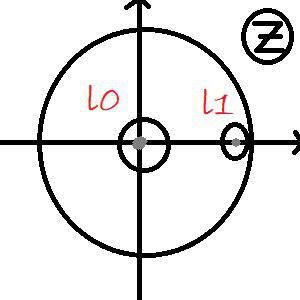
\includegraphics{lec33_1}
	\end{center}
	
	Отделяя особые точки и учитывая лемму об 
	интеграле от ФКП для многосвязной ФКП имеем 
	$I = I_0 + I_1$, где 
	\[
	I_0 = 
	\oint\limits_{l_0}\dfrac{\cos z}{z^2(z - \pi)} 
	dz=
	\oint\limits_{l_0}\dfrac{\frac{\cos z}
		{z-\pi}}{z^2} dz
	= \left[
	\begin{array}{l}
	f(z) = \dfrac{\cos z}{z-\pi} \\
	n = 1
	\end{array}
	\right] = 
	2\pi i \left( \dfrac{\cos z}{z-\pi}\right)'
	\bigg|_{z=0}=
	\]
	\[= -2\pi i \cdot \dfrac{\cos z + 
		(z - \pi) \sin z}{(z-\pi)^2}\bigg|_{z=0}=
	-2\pi i \cdot {1}{\pi ^2} = -\dfrac{2i}{\pi}.
	\]
	\[
	I_1 = \oint_{l_1} \dfrac{\frac{\cos z}{z^2}}
	{z-\pi} dz = 2 \pi i \cdot \left(
	\dfrac{\cos z}{z^2}
	\right) |_{z=\pi} = 2\pi i \cdot \dfrac{-1}{\pi^2}
	=\dfrac{-2i}{\pi}.
	\]
	Т.~е.
	\[
	I = I_0 + I_1 = -\dfrac{4i}{\pi}.
	\]
\end{exmp}

\section{Некоторые приложения интегрального
	представления производных ФКП}

Далее $f(z)$, дифференцируемую для $\forall z \in \C$
будем называть \emph{целой ФКП}.
\begin{thm}[Лиувилль]
	Если целая $f(z)$ является ограниченной в $\C$,
	то есть
	\begin{equation}
	\label{lec33:11}
	\exists M = const > 0 : \abs{f(z)}
	\leq M,\ \forall z \in \C, 
	\end{equation}
	то тогда $f(z)$ тождественно равна константе.
\end{thm}
	
\begin{proof}
	Для фиксированного $ z \in \C $ и $ R > 0 $ рассмотрим 
	в плоскости \textcircled{t} окружность 
	\[ l_R = \{ t \in \C\ |\ \abs{t - z} = R\}. \] 
	Тогда из \eqref{lec33:7} при $ n = 1 $ имеем:
	\[
	f'(z) = \dfrac{1}{2\pi i} \oint\limits_{l_R} 
	\dfrac{f(t)}{(t - z)^2} dt \implies
	\abs{f'(z)} \leq \dfrac{1}{2\pi}
	\oint\limits_{l_R} \dfrac{\abs{f(t)}}{\abs{t - z}^2}
	\abs{dt} \leq
	\begin{bmatrix}
		\abs{f(t)} \leq M \\
		\abs{t - z} = R
	\end{bmatrix} \leq \dfrac{M}{2\pi R^2}
	\oint\limits_{l_R} \abs{dt} =\]
	\[=
	\dfrac{M}{2\pi R^2}\cdot\text{Длина }
	l_R = \dfrac{M}{2\pi R^2} \cdot 2\pi R = \dfrac{M}{R}.
	\]
	Из полученного неравенства следует, что $ \abs{f'(z)} \leq 
	\dfrac{M}{R} $. В силу того, что $ M = const $ не 
	зависит от $ R > 0 $, при $ R \to +\infty $ имеем:
	\[
	\abs{f'(z)} \leq 0 \implies 
	\abs{f'(z)} = 0 \implies 
	f'(z) = 0.
	\] Т.~е. $f(z) = const \in \C$ в силу критерия постоянства ФКП.
\end{proof}
\begin{rem}
	Теорема Лиувилля показывает, что если ФКП $ f(z) \not\equiv const $,
	то в $ \C $ у неё, возможно, есть особенности, т.~к.
	она не может быть аналитической всюду в $ \C $.
\end{rem}

С другой стороны, целые ФКП $ \not\equiv const $ не могут быть ограничены в $ 
\C $.
Отсюда, в частности, следует, что бесконечные дифференцируемые ФКП
является целыми и неограниченными, в отличие от действительного 
случая. Например, для $ \sin x $ и $ \cos x$ при $x \in \R $ верно $ \abs{\sin 
x} \leq 1,\ \abs{\cos x} \leq 1,\ \forall x \in \R $. 
Если $x \in \C$ то, несмотря на выполнение основного тригонометрического 
тождества, 
из него не следует ограниченность комплексных тригонометрических функций $ 
\sin z,\ \cos z $. Например, если $ z = iy $, то
$ \cos z = \cos iy = \ch y
\underset{y \to \infty}{\to} \infty$.

\begin{crl}[основная теорема алгебры]
	Если многочлен ${P_n(z) = c_0 + c_1z + \dots + c_nz^n}$, $c_k \in \C,\
	k = \overline{0, n},\ c_n \neq 0 $, имеет $ n \geq 1 $, то уравнение $ P_n(z) 
	= 0 $ имеет хотя бы один комплексный корень.
\end{crl}
\begin{proof}
	Пусть $ P_n(z) \neq 0\quad \forall z \in \C $.
	Тогда $ f(z) = \dfrac{1}{P_n(z)} $ не имеет особенностей в $ \C $ 
	и будет дифференцируема для $ \forall z \in \C,\
	f'(z) = -\dfrac{P_n'(z)}{P_n(z)^2} $. Значит, 
	$ f(z) $~--- целая ФКП.
	
	Учитывая, что $ f(\infty) = 0$, получаем, что
	\[\exists R = const > 0\quad \forall z \in \C,\ |z| \ge R \implies f(z) 
	\text{ ограничена}.\] Кроме того, по теореме Вейерштрасса, $f(z)$ будет 
	ограничена и на компакте $ \abs{z} \leq R $.
	Значит, $ f(z) $ ограничена на $ \C $ и поэтому по теореме Лиувилля следует, 
	что
	$ f(z) = const \neq 0 \implies P_n(z) = \dfrac{1}{f(z)} = const $, 
	что противоречит тому, что $ P_n(\infty)  = \infty $. Поэтому $ 
	{\exists z_0 \in \C: P_n(z_0) = 0}$.
\end{proof}

Отметим, что если дальше разложить $ P_n(z) = (z - z_0)Q_{n - 1}(z), $ 
то в случае $ n \geq 2 $ у $ Q_{n - 1}(z),\ n - 1 \geq 1 $, 
также $ \exists z_1 : Q_{n - 1}(z_1) = 0 $ и т.~д.
В конце концов получим, что любой многочлен в $ \C $ степени $ n \in \N $ 
имеет 
ровно $ n $ комплексных корней с учётом их кратности.

\begin{thm}[Морера]
	Если $ f(z) $ непрерывна в области $ D $ и для любого кусочно-гладкого 
	замкнутого контура $ l \subset D $ имеем
	\begin{equation}
	\label{lec33:12}
	\oint\limits_l f(z) dz = 0,
	\end{equation}
	то тогда $ f(z) $ аналитична в $ D $.
\end{thm}
\begin{proof}
	Для фиксированного $ z_0 \in D $ и
	$ \forall z \in D $ рассмотрим 
	\begin{equation}
	\label{lec33:13}
	\Phi(z) =
	\int\limits_{z_0}^{z} f(t) dt.
	\end{equation}
	Функция \eqref{lec33:13} корректно определена в том смысле, 
	что \eqref{lec33:13} не зависит от пути интегрирования между $z_0$ и $z$:
	\begin{center}
	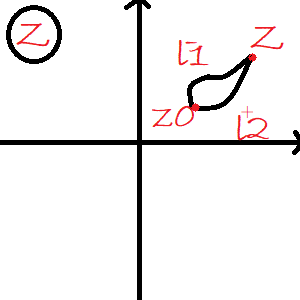
\includegraphics{lec33_2}
	\end{center}
	Пусть $l_0 = l_2^+ \cup l_1^+$. Тогда
	\[
	\oint\limits_{l_0} f(t) dt = 0 \implies
	\int\limits_{l_1^+} f(z) dz +
	\int\limits_{l_2^+} f(z) dz = 0 \implies 
	\int\limits_{l_1^+} f(z) dz =
	\int\limits_{l_2^-} f(z) dz.
	\]
	Так же, как и в теореме о существовании первообразной
	ФКП для \eqref{lec33:13} получаем, что $ \exists \Phi'(z) = f(z) $. 
	Из аналитичности $ \Phi(z) \implies $ 
	аналитичность $ \Phi'(z) \implies $
	аналитичность $ f(z) $ в $ D $.
\end{proof}
\begin{rem}
	По своей сути, теорема Мореры является обратной
	к интегральной теореме Коши.
\end{rem}

\end{document}
